\documentclass{article}
\usepackage{amsmath}
\usepackage{fullpage}
\usepackage{graphicx}

\title{Spherical Coordinates}
\author{M. en C. Reinaldo Zapata}

\begin{document}
\maketitle

\section*{Spherical coordinates} % (fold)
\label{sec:spherical_coordinates}

\begin{align*}
r &= \sqrt{x^{2} + y^{2} + z^{2}} & & r \geq 0\\
\theta &= \arccos \left( \frac{z}{r} \right) & 0 \leq &\theta \leq \pi \\
\varphi &= \arctan \left( \frac{y}{x} \right) & 0 \leq &\theta \leq 2\pi \\ \\ 
x &= r \, \sin \theta \, \cos \varphi \\
y &= r \, \sin \theta \, \sin \varphi \\
z &= r \, \cos \theta
\end{align*}

\begin{figure}[h]
    \centering
    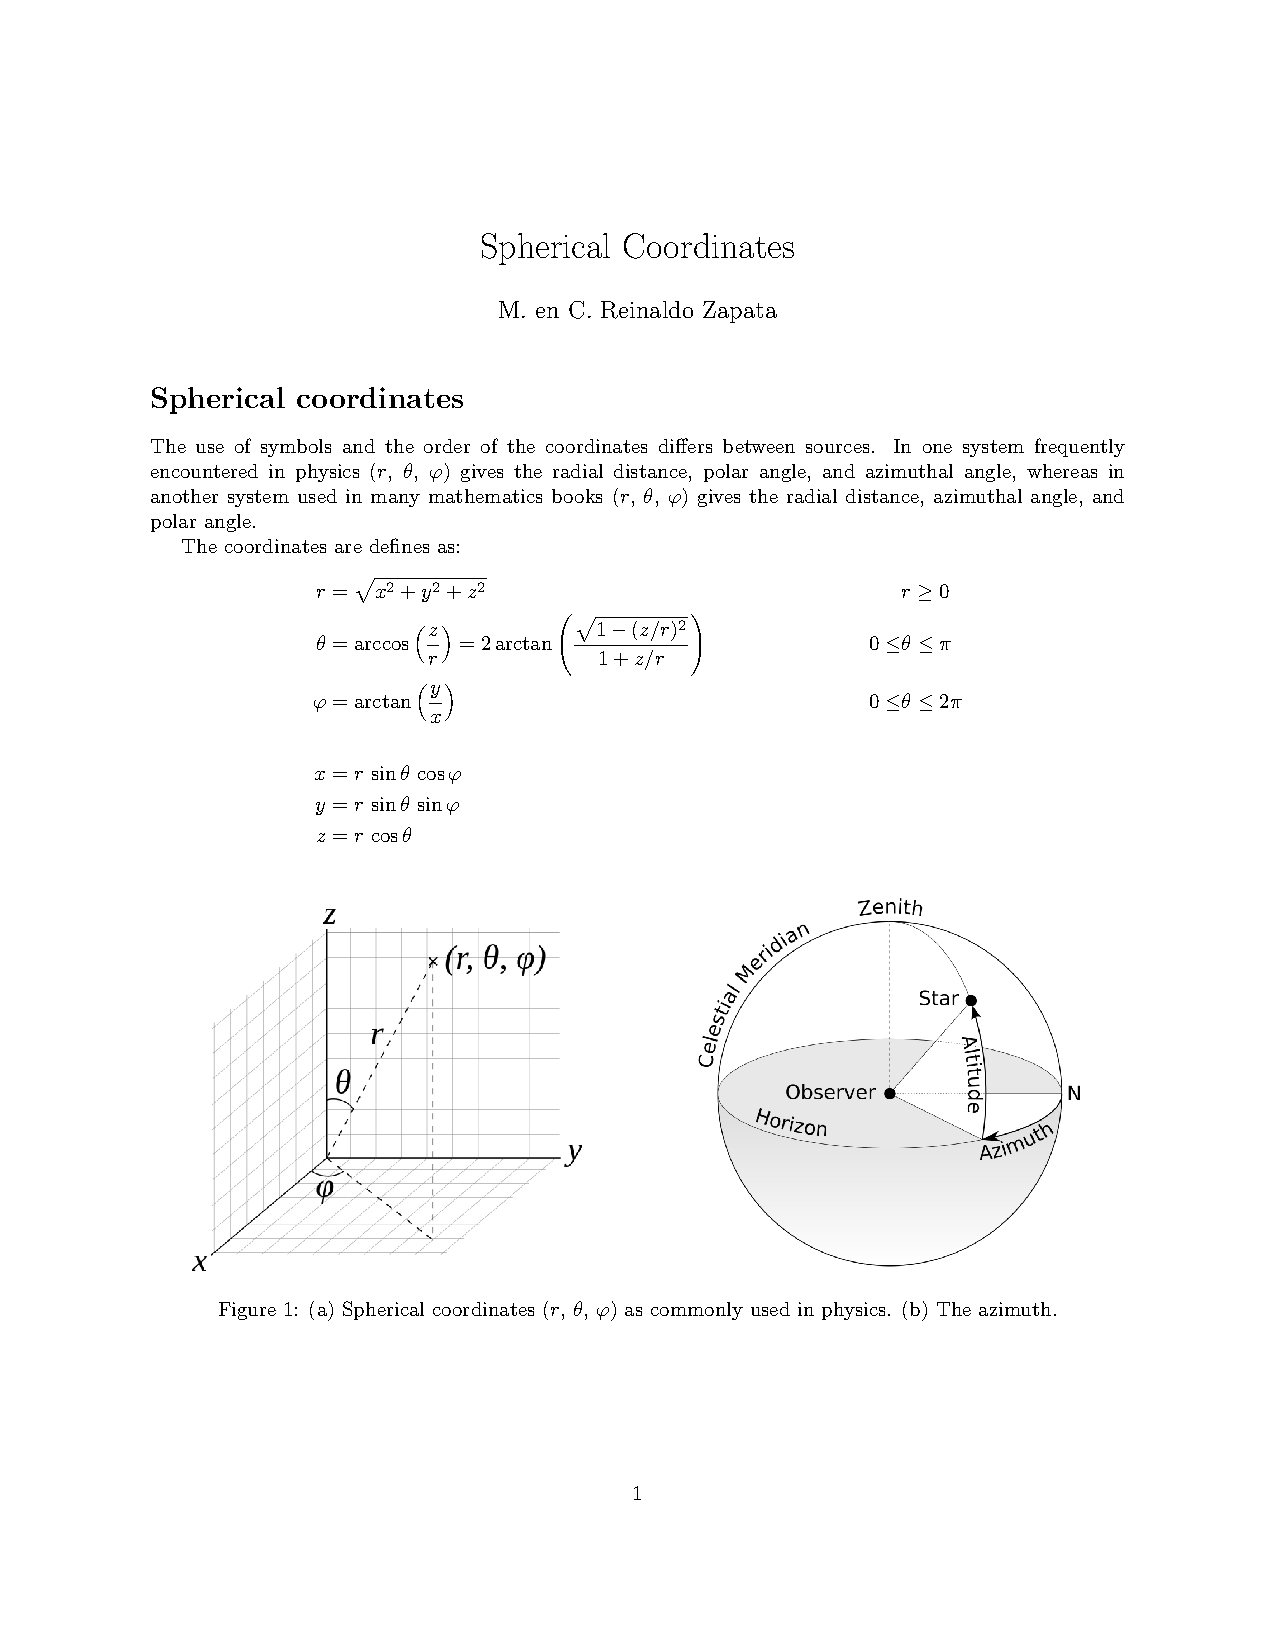
\includegraphics[width=0.4\textwidth]{spherical_coordinates}
    \caption{Spherical Coordinates.}
    \label{fig:spherical coordinates}
\end{figure}

\tt{acos =  atan2(sqrt(1-x*x), x) }


% section spherical_coordinates (end)


\end{document}
